\section{Základní nelinearity a popis nelineárních systémů (popis statických a dynamických nelineárních systémů,
vliv parazitních nelinearit na průběh regulačního děje)}



\subsection{bez dynamiky}
Systém reaguje na odezvu okamžitě, nebo je jeho časová kosatanta výrazně nižší něž zyblé čas. konstanty.
Dělí se na :

\begin{itemize}
    \item bez paměti
    \item s pamětí
\end{itemize}

\subsubsection*{nelinearita bez paměti}

Dá se vyjádřit jako funkce 
\begin{equation}
    y=f(u)
\end{equation}

Na zákadě aktuální hodoty se určí výstup. Dá se jednoduše linearizovat rozvojem da taylorovy řady, nebo do polynomu.
posána funkcí, grafem, tabulkou.
\\
např. :  saturace, tření\dots
\\
\\
\subsubsection*{nelinearita z pamětí}
Výstup zálezí i na předchozích satvech, nelze jednoduše popsat jako funkce, často se popisuje slovně nebo jako algorytmus.
\\
např.: vůle v převodech, relé s hysterezí

\subsection*{Základní nelinearity}

\subsubsection*{nasycení(saturace)}
\begin{itemize}
    \item nejběžnejší nelinearita (obsahuje ji vpodstatě každý reálný systém)
    \item dá se s ní pracovat jako s po částech lineární funkcí
    \item pokud zajistíme že se systém nedosatne z <b,a> lze prát jako lin. f-ce 
    \item např.: nádrž co přeteče
    \item (je jedním z faktorů pro vzik wind up jevu)
    \item bez paměti
\end{itemize}
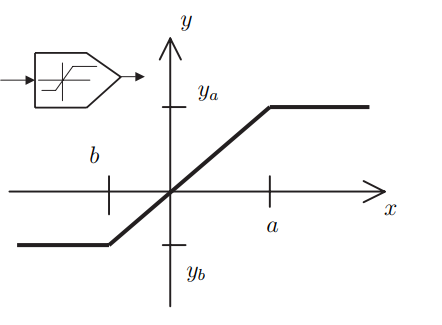
\includegraphics[]{img/saturace.png}

\subsubsection*{necitlivost}
\begin{itemize}
    \item nejčasttěji u mech systémů (projev tření a mech. nepřesností)
    \item např.: DC motor se roztočí až od určitého napětí
    \item občas se vkládá do reg. umělěle aby se omezili oscilace
    \item po částech lineární (většinou)
    \item bez paměti
\end{itemize}
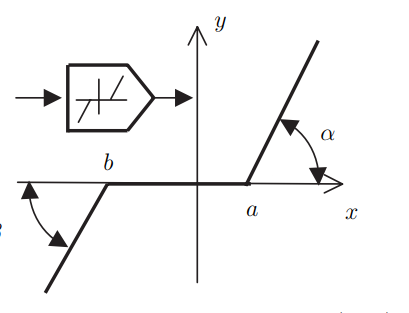
\includegraphics{img/necitlivost.png}

\subsubsection*{vůle v převodech (hystereze)}
\begin{itemize}
    \item při změně pohybu chíli trvá než se něco začne dít
    \item v převodovkách , nebo při magnetizaci železa (hysterezní symčka- v otázce MVE mag. měřemí)
    \item v převodovce lze odstarnit tak že druhý motor tlačí vždycky proti
    \item rádi se na to ptají
    \item vetšinou nelze linearizovat
    \item s pamětí
\end{itemize}
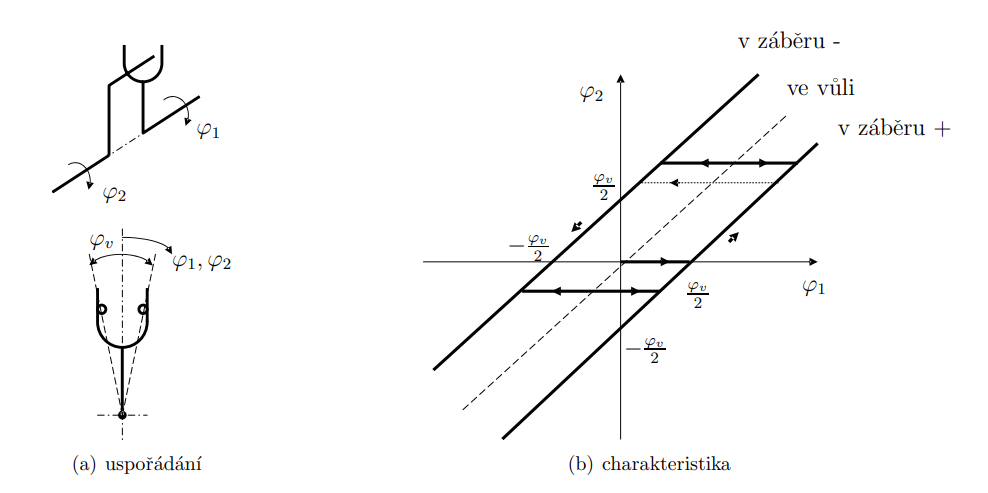
\includegraphics{img/vule.png}

\subsubsection*{tření}
\begin{itemize}
    \item v mech systémech
    \item špatně se linearizuje v oklí 0
    \item bez paměti
\end{itemize}
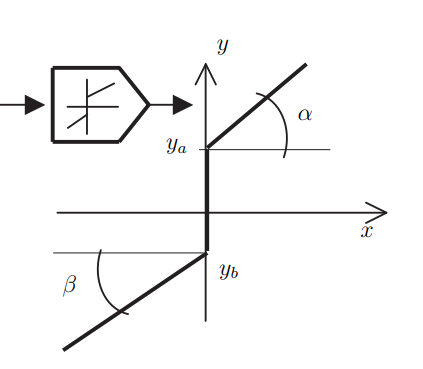
\includegraphics{img/treni.png}

\subsection*{releové charakteistiky}
\begin{itemize}
    \item s pamětí i bez
    \item požití jako regulátor
\end{itemize}
\includegraphics*{img/rele.png}


\subsection{s dynamikou}
popsány stavovými rovnicemi:
\[
    \frac{dx}{dt}=f(x,u)\]
    \[y=g(x,u)\]


\begin{itemize}   
    \item časově variantní
    \item časově invariantí (paramtry se v čase nemění)
\end{itemize}

\section{Ustálené chování nelineárních dynamických systémů (rovnovážné stavy, mezní cyklus, metoda
harmonické rovnováhy, stabilita mezního cyklu)}

\subsection{rovnovážný stav}
Stav systému, ktrý se v čase nemění. x=0 Průmět stavové trajekotrie je bod. Určíme
ho jako \[ \dot{x} = 0 \]
Systém může mít o vice rovnocážných stavů, také nemusí mít žádný.

Rovnovážné stavy mohu být:
\begin{itemize}
    \item izolované - pokud kolem něj exzistuje jeho maůlé okolí ve kterém se nenachází dlaší rovnovážný stav.
    \item neizolované
\end{itemize}

U rovnovážných stavů pak můžeme řešit jejich stbilitu pokud se systém po drobném vychýlení do rovanážného 
satvu vrátí je rovnovážný stav stabilní.
O stabilitě/nestabilitě lze rohodnou lineazizací rozvojem do taylorovy řady (podle polohy pólů náhrady)


\subsubsection{mezní cyklus}

